%!TEX root = ../main.tex

Apesar do esforço dispendido em pesquisas sobre o \textit{DNS} para \textit{MANETs},
ainda não existe consenso sobre qual o melhor modelo a ser 
adotado. Enquanto que algumas propostas exigem modificações drásticas no 
protocolo de resolução de nomes já existente -- impedindo assim que 
implementações atuais possam ser reutilizadas -- outras deixam muito a desejar 
no quesito de energia consumida, sobrecarregando um nó da rede e usando-o como
 servidor.

Existem três casos principais para os quais as especificações de DNS para 
\textit{MANETs} precisam encontrar uma solução. O primeiro é o caso de não existir 
nenhum servidor, ou existirem múltiplos servidores na rede. Cabe ao protocolo 
definir como o primeiro servidor deve ser criado, como vai operar em relação 
aos demais, e se pode haver mais de um servidor. O segundo caso diz respeito à 
configuração dinâmica; diferente das redes com infraestrutura, não é possível 
ter um \textit{Master File} com nomes e traduções à disposição do Servidor de 
Nomes. Além disso, nomes e endereços associados aos nomes podem mudar muito em 
uma rede. O terceiro caso a ser tratado é o conflito de nomes -- que no caso de 
\textit{MANETs} pode ocorrer tanto no momento da escolha de nomes quanto na fusão
 de duas redes. Segundo as especificações do DNS \cite{rfc1035}, cada 
 identificador dentro de uma rede deve ser único. A seguir são descritos os 
 protocolos existentes na literatura e qual a sua solução para os problemas descritos.

\section{Context-Based Name Resolution Service}
\label{context-based}

    Apesar da falta de detalhes técnicos sobre a proposta, \cite{context-dns}
    traz um protocolo mais adequado às MANETs. Como o nome
    sugere, o \textit{Context-Based Resolution Service} é um protocolo que usa
    informações de contexto para a tradução de nomes. O artigo define \emph{nome}
    como a descrição de um objeto e \emph{endereço} como a localização física do
    objeto. Ao mapeamento do nome para o endereço dá-se o nome de \emph{resolução}.
    
    \cite{context-dns} ainda apresenta o conceito de \textit{namespaces}, que são
    nomes válidos dentro de um certo contexto. Assim, uma aplicação pode reconhecer
    um \textit{namespace} para vários contextos, vários \textit{namespaces} para
    um contexto, ou um \textit{namespace} para um contexto (figura \ref{namespaces}).
    
    \begin{figure}[h!]
        \centering
        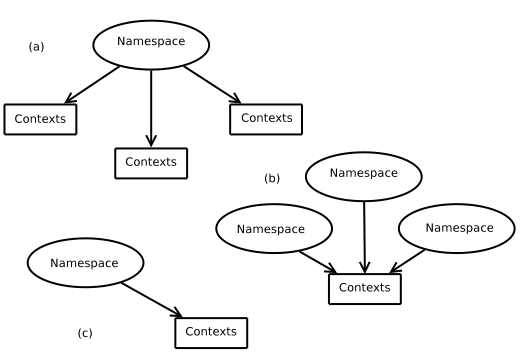
\includegraphics[width=0.8\textwidth]{figures/contexts}
        \caption{Contextos e \textit{namespaces}}
        \label{namespaces}
    \end{figure}
    
    Existem muitas sugestões no artigo sobre o que podem ser os contextos, mas a
    solução mais recorrente no texto é o uso de sensores e observadores externos
    para determinar o contexto da rede. Para obter um ambiente apropriado, cria-se
    uma camada de descrição de contexto que pode fazer uso de ontologias que
    descrevem conceitos e relações entre objetos em certos contextos. Os pré-requisitos
    para tal são
    \begin{inparaenum}[(i)]
        \item uma linguagem de descrição de ontologias,
        \item um repositório,
        \item um raciocinador, para interpretar as relações entre ontologias e
        informações de contexto (\textit{tags}).
    \end{inparaenum} 
    Assim, de forma genérica, o processo de tradução ocorre em duas fases
    (figura \ref{translation}): a primeira de obtenção de contexto; a segunda
    de tradução dentro do \textit{namespace} daquele contexto.
    
    \begin{figure}[h!]
        \centering
        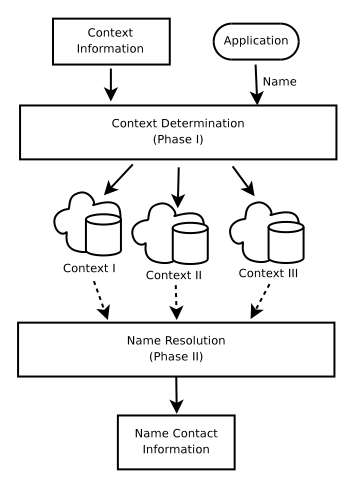
\includegraphics[width=0.5\textwidth]{figures/translation}
        \caption{Tradução em duas fases}
        \label{translation}
    \end{figure}
    
    Mesmo definindo vários contextos e várias estratégias de tradução, o artigo
    não especifica nenhum caso e nem onde os mapeamentos das traduções seriam
    alocados na rede, nem como ou se a rede funcionaria dentro do princípio do
    \textit{Zeroconf} \cite{zeroconf}. No entanto, o que os pré-requisitos dão
    a entender é que dispositivos com baixo poder de memória e processamento
    não são bem vindos na rede. Também fica claro que os autores exigem que
    existam certas condições que podem não ser encontradas tão facilmente em
    MANETs, como a existência de repositórios. Uma vez que um repositório exige
    um servidor confiável e não se pode assumir confiabilidade em conexão entre
    nós em uma rede MANET, como explicado no capítulo \ref{intro}. Questões como
    tratamento de conflito de nomes e regras de desconexão também não são tratados.
    
    Por esses motivos, o \textit{Context-Based Name Resolution Service} pode não
    ser uma solução totalmente adequada à MANETs, apesar de representarem
    uma nova abordagem e considerável melhoria do protocolo DNS.

\section{Link Local Multicast Name Resolution}

    \textit{Link Local Multicast Name Resolution} (LLMNR) \cite{llmnr} é uma
    extensão do DNS tradicional (DNSExt) e não se propõe a substituir por
    completo o DNS. O LLMNR é limitado a pequenas redes, funciona sobre
    \textit{peer-to-peer} (p2p) e sua especificação esclarece que deve ser usado
    somente em situações em que o DNS não está disponível ou não é compatível.
    
    \cite{llmnr} sugere que a configuração dos servidores seja feita através de
    DHCP4 ou DHCP6, mas também explica que esses não são os únicos métodos de
    configurar os servidores. Qualquer nó da rede pode ser um servidor, mas não
    existe obrigação para que nenhuma máquina o seja. As consultas de nomes são
    feitas via broadcast (caso geral) ou unicast (caso em que um nó já conhece o
    servidor autoritativo para o nome que procura), e a resposta é sempre em unicast.
    
    Conflitos de nomes são detectados através de consultas normais de tradução. Se
    um nó receber duas respostas diferentes de servidores diferentes para uma
    requisição, esse nó deve reenviar essa requisição com um bit a mais ligado
    no pacote, indicando que os servidores devem analisar essa consulta e não
    devem respondê-la. Servidores também podem verificar periodicamente se existe
    duplicidade para os nomes dos quais são autoritativos, mas não existe
    obrigatoriedade nem período máximo para essa tarefa.
    
    Uma vez detectado o conflito, os servidores autoritativos para aquele nome
    devem tomar uma atitude para corrigir o problema. Se ambos os servidores
    estiverem se declarando autoritativo para a mesma tradução, ou seja, ambos
    estão mapeando o mesmo nome para o mesmo nó, é considerado que não há conflito,
    mas apenas um deve continuar sendo autoritativo. Caso cada um dos servidores
    esteja mapeando uma tradução diferente, cada um deles faz uma análise lexográfica
    do IP de cada nó conflitante: o nó com IP lexograficamente menor (indicando
    que ele está há mais tempo na rede) tem direito a usar aquele nome, e a
    tradução que aponta para o nó com IP lexograficamente maior é ignorada. Um log
    é gerado apontando a ação tomada, e esse nó pode ser manualmente reconfigurado
    pelo administrador da rede.
    
    Como a própria especificação explica, essa solução não é um substituto para
    o DNS. Apesar de oferecer quase todos os serviços disponibilizados pelo DNS
    tradicional, o LLMNR se limita a redes pequenas, necessita de servidores e
    assume que existe um nível mínimo de confiabilidade na rede.

\section{Bonjour}
\label{Bonjour}

    Criado pela \textit{Apple} primeiramente com o nome \textit{Rendezvous}, o 
    \textit{Bonjour} implementa o \textit{Zero Configuration Network} 
    (\textit{zeroconf}) \cite{zeroconf}, que é uma especificação que engloba vários
    serviços para redes com configuração dinâmica, entre eles, o 
    \textit{Multicast DNS} (\textit{mDNS}) \cite{mdns}. Apesar do seu código ser 
    aberto, sua documentação é limitada, portanto as especificações descritas aqui
    são conclusões tiradas a partir de testes realizados com o protocolo.  

\label{MDNS}
 
    O protocolo \textit{Bonjour} é completamente reativo e isso se aplica também
    à resolução dos nomes na rede, usando o \textit{mDNS}. Quando uma nova máquina
    entra na rede, ela anuncia via \textit{broadcast} seu nome, seu endereço 
    \emph{IP} e os serviços que disponibiliza. As outras máquinas da rede 
    atualizam suas tabelas de tradução de nomes e serviços. Esse método de 
    associar nomes e serviços é chamado \textit{DNS Service Discovery} 
    (\textit{DNS--SD}) \cite{dnssd}. Caso o nome escolhido pela nova máquina 
    já exista na rede, essa máquina tem um número adicionado ao final do seu 
    nome. Por exemplo, se um nó tenta entrar na rede com o nome \emph{foo}, mas
    esse nome já está em uso, uma máquina que já pertence à rede (e atua como
    \textit{bootstrap}) envia uma mensagem a essa nova máquina avisando que seu
    nome está sendo alterado para \emph{foo1}.

    Uma máquina nova na rede tem sua tabela de tradução vazia e quando 
    precisar de algum nome ou serviço envia sua requisição para toda a rede,
    via \textit{multicast}. Toda máquina na rede que roda o protocolo
    \textit{Bonjour} é um servidor de nomes, e pode responder a essa 
    requisição se tiver a tradução requisitada. A nova máquina atualiza sua 
    tabela com os resultados recebidos.

    Se uma máquina adicionar algum serviço na rede, deve fazer um anúncio via
    \textit{multicast} para alertar as outras máquinas. No entanto, não há 
    nenhum aviso se algum serviço for retirado, assim como não há nenhuma 
    regra no protocolo para um nó sair da rede. Apesar de todas as máquinas 
    enviarem anúncios periódicos dos serviços que disponibilizam, as entradas
    nas tabelas não possuem um \textit{time--to--live}, de modo que os serviços
    e nomes de máquinas que não estão mais na rede persistem indefinidamente.

    Essa abordagem funciona muito bem para redes pequenas, mas pode apresentar
    problemas de escalabilidade, não é apropriada para equipamentos com 
    processamento e memória limitados. Por limitações nos testes, não foi possível
    descobrir se esse protocolo funciona quando é necessário fazer roteamento,
    isto é, quando a fonte e o destino das mensagens estão a mais de um salto
    de distância. O protocolo \textit{Bonjour} foi feito visando ambientes 
    corporativos médios, por isso não existe a preocupação com escalabilidade.

    Pelo fato de definir todas as máquinas da rede como servidores, exigir um
    anúncio periódico de serviços, e não lidar com conflitos decorrentes da união
    de redes preexistente, o \textit{Bonjour} não é um protocolo ideal para redes
    MANET, apesar de se destacar em redes locais de pequeno e médio porte com
    \textit{zeroconf}.


\section{Modified Centralized DNS}
\label{MCDNS}

    O \textit{Modified Centralized DNS}, ou \textit{Manet DNS}, como é referenciado
    no seu artigo \cite{mcdns}, propõe implementar exatamente o que geralmente é
    evitado em projetos de protocolos para MANETs: uma solução centralizada.
    O artigo alega que as afirmações de que um protocolo centralizado em uma MANET
    apenas apontam uma tendência esperada, mas que essa proposta nunca foi testada.
  
    O \textit{Manet DNS} se assemelha muito ao funcionamento atual do DNS para 
    redes com infraestrutura, apesar de respeitar as normas da rede \textit{Zeroconf}
    \cite{zeroconf}, o que inclui configuração dinâmica, que no caso acontece sob
    demanda. Um Servidor de Nomes (NS) só é criado se uma máquina precisar do 
    serviço de tradução de nomes e ainda não existir um servidor na rede. Nesse 
    caso, essa máquina se torna um servidor, e deve mandar anúncios periódicos à
    rede para deixar clara sua presença. Se alguma máquina não receber esse
    anúncio por um período de tempo, interpreta que não existe mais Servidor de 
    Nomes em seu alcance, seja por quebra da rede -- pela mobilidade dos nós --,
    ou por que o antigo servidor foi desligado.

    Se um nó novo na rede ainda não sabe da existência de um servidor, deve enviar
    um broadcast requisitando um servidor (figura \ref{centralized}). Se essa
    consulta não revelar nenhum servidor de nomes, o nó se torna um servidor de
    nomes.
    
    \begin{figure}[h!]
        \centering
        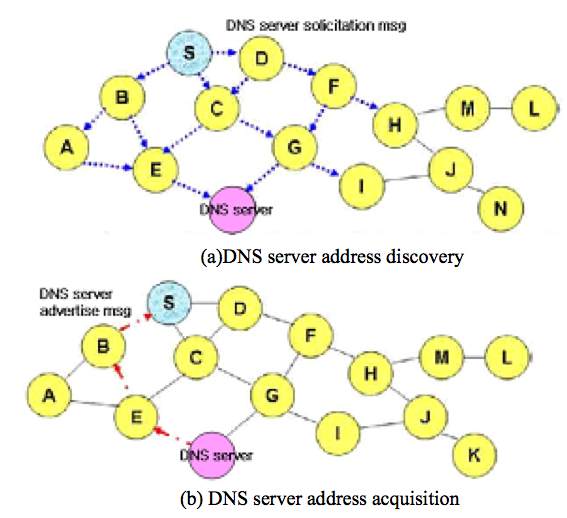
\includegraphics[width=0.5\textwidth]{figures/centralized}
        \caption{Nó descobrindo presença de um servidor na rede}
        \label{centralized}
    \end{figure}

    Quando um NS é criado, a máquina envia um 
    \textit{broadcast} à rede pedindo que todas as máquinas lhe enviem suas 
    informações. As outras máquinas da rede respondem a essa requisição com seu 
    nome e endereço, via \textit{unicast}, e já registram que existe um NS na rede.
    Caso exista um conflito de nomes, o NS aceita o nome da primeira máquina que
    respondeu à requisição e envia uma mensagem para a segunda pedindo
    para que escolha outro nome. Esse processo pode se repetir até um dado número
    de vezes (configurável) e se o conflito persistir, o NS escolhe um nome 
    aleatório para essa máquina.
  
    No caso de haver mais de um servidor na rede, os NS existentes precisam
    chegar a um consenso sobre qual máquina vai continuar com o serviço. Essa
    decisão se da comparando os IP's dos servidores; assim definindo
    qual tem maior prioridade sobre os demais. O servidor com maior prioridade recebe
    a tabela de tradução de nomes dos servidores com menor prioridade, e deve resolver
    eventuais conflitos de nomes que essa fusão possa causar.
  
    Se uma máquina \textbf{A}, após conseguir a tradução de uma máquina \textbf{B},
    descobrir que \textbf{B} não está mais na rede, \textbf{A} pode enviar essa 
    informação ao servidor que guarda a tradução do nome de \textbf{B}. Se o servidor
    receber essa informação repetidamente, retira a máquina \textbf{B} de sua 
    tabela de tradução, considera que essa máquina não está mais disponível na 
    rede, e o nome \textbf{B} está livre para ser usado.
  
    Os testes realizados pelo autores do protocolo revelam um desempenho melhor
    em relação ao \textit{Multicast DNS} nos quesitos tempo de resposta e tráfego
    gerado por mensagens de controle. No entando os números sobre o consumo de 
    energia do servidor não estão disponíveis e o tempo de execução da simulação
    -- 100 segundos -- é considerado pequeno para esse tipo de teste.
    
    Ainda, esse protocolo pode não ser adequado para redes com dispositivos
    limitados. Um único servidor, além de representar um ponto único de falha,
    pode também ser um gargalo no caso da rede ser muito ativa e a bateria do
    dispositivo escolhido como servidor pode ser consumida em um curto tempo.